\begin{center}
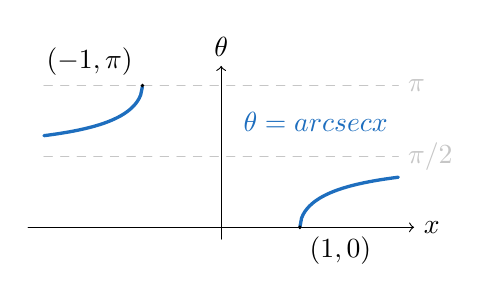
\begin{tikzpicture}[scale=1.0, line cap=round, line join=round]
  \definecolor{trigblue}{RGB}{30,110,190}
  \draw[->] (-2.45,0)--(2.45,0) node[right] {$x$};
  \draw[->] (0,-0.15)--(0,2.05) node[above] {$\theta$};
  \draw[gray!45,dashed] (-2.25,1.8)--(2.25,1.8) node[right] {$\pi$};
  \draw[gray!45,dashed] (-2.25,0.9)--(2.25,0.9) node[right] {$\pi/2$};
  \draw[very thick,trigblue,domain=1:2.25,samples=60]
    plot ({\x},{1.8*acos(1/\x)/180});
  \draw[very thick,trigblue,domain=-2.25:-1,samples=60]
    plot ({\x},{1.8*acos(1/\x)/180});
  \fill (1,0) circle (0.025) node[below right] {$(1,0)$};
  \fill (-1,1.8) circle (0.025) node[above left] {$(-1,\pi)$};
  \node[trigblue] at (1.2,1.34) {$\theta=\operatorname{arcsec} x$};
\end{tikzpicture}
\end{center}
